\documentclass{standalone}
\usepackage{tikz}
\usetikzlibrary{patterns, positioning}

\begin{document}
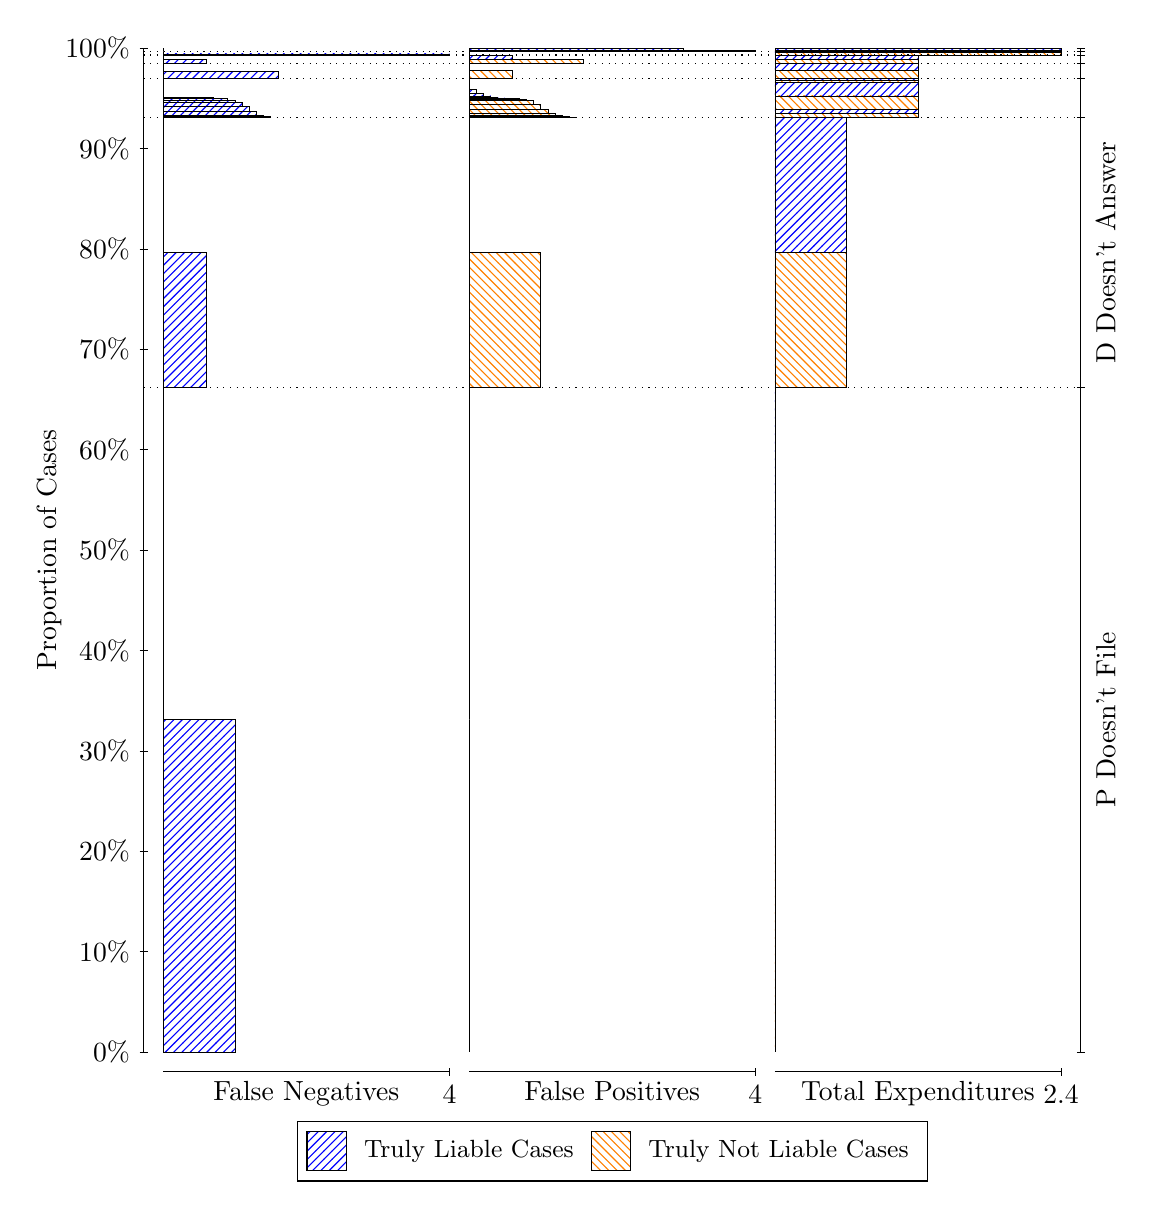
\begin{tikzpicture}
\draw[black, very thin] (1.5,1.75) -- (1.5,14.5);
\node[rotate=90, anchor=center] at (0.3, 8.125) {Proportion of Cases};
\draw[black, very thin] (1.45,1.75) -- (1.55,1.75);
\node[anchor=east] at (1.45, 1.75) {0\%};
\draw[black, very thin] (1.45,3.025) -- (1.55,3.025);
\node[anchor=east] at (1.45, 3.025) {10\%};
\draw[black, very thin] (1.45,4.3) -- (1.55,4.3);
\node[anchor=east] at (1.45, 4.3) {20\%};
\draw[black, very thin] (1.45,5.575) -- (1.55,5.575);
\node[anchor=east] at (1.45, 5.575) {30\%};
\draw[black, very thin] (1.45,6.85) -- (1.55,6.85);
\node[anchor=east] at (1.45, 6.85) {40\%};
\draw[black, very thin] (1.45,8.125) -- (1.55,8.125);
\node[anchor=east] at (1.45, 8.125) {50\%};
\draw[black, very thin] (1.45,9.4) -- (1.55,9.4);
\node[anchor=east] at (1.45, 9.4) {60\%};
\draw[black, very thin] (1.45,10.675) -- (1.55,10.675);
\node[anchor=east] at (1.45, 10.675) {70\%};
\draw[black, very thin] (1.45,11.95) -- (1.55,11.95);
\node[anchor=east] at (1.45, 11.95) {80\%};
\draw[black, very thin] (1.45,13.225) -- (1.55,13.225);
\node[anchor=east] at (1.45, 13.225) {90\%};
\draw[black, very thin] (1.45,14.5) -- (1.55,14.5);
\node[anchor=east] at (1.45, 14.5) {100\%};

\draw[black, very thin] (13.4,1.75) -- (13.4,14.5);
\draw[black, very thin] (13.35,1.75) -- (13.45,1.75);
\node[anchor=west] at (13.35, 1.75) {};
\draw[black, very thin] (13.35,10.19) -- (13.45,10.19);
\node[anchor=west] at (13.35, 10.19) {};
\draw[black, very thin] (13.35,13.616) -- (13.45,13.616);
\node[anchor=west] at (13.35, 13.616) {};
\draw[black, very thin] (13.35,14.114) -- (13.45,14.114);
\node[anchor=west] at (13.35, 14.114) {};
\draw[black, very thin] (13.35,14.305) -- (13.45,14.305);
\node[anchor=west] at (13.35, 14.305) {};
\draw[black, very thin] (13.35,14.411) -- (13.45,14.411);
\node[anchor=west] at (13.35, 14.411) {};
\draw[black, very thin] (13.35,14.456) -- (13.45,14.456);
\node[anchor=west] at (13.35, 14.456) {};
\draw[black, very thin] (13.35,14.5) -- (13.45,14.5);
\node[anchor=west] at (13.35, 14.5) {};

\draw[black, very thin, pattern color=blue, pattern=north east lines] (1.75,1.75) rectangle (2.6583,5.97);
\draw[black, very thin, pattern color=orange, pattern=north west lines] (1.75,5.97) rectangle (1.75,10.19);
\draw[black, very thin, pattern color=blue, pattern=north east lines] (1.75,10.19) rectangle (2.295,11.901);
\draw[black, very thin, pattern color=orange, pattern=north west lines] (1.75,11.901) rectangle (1.75,13.616);
\draw[black, very thin, pattern color=blue, pattern=north east lines] (1.75,13.616) rectangle (3.1125,13.632);
\draw[black, very thin, pattern color=blue, pattern=north east lines] (1.75,13.632) rectangle (3.0217,13.643);
\draw[black, very thin, pattern color=blue, pattern=north east lines] (1.75,13.643) rectangle (2.9308,13.694);
\draw[black, very thin, pattern color=blue, pattern=north east lines] (1.75,13.694) rectangle (2.84,13.756);
\draw[black, very thin, pattern color=blue, pattern=north east lines] (1.75,13.756) rectangle (2.7492,13.811);
\draw[black, very thin, pattern color=blue, pattern=north east lines] (1.75,13.811) rectangle (2.6583,13.839);
\draw[black, very thin, pattern color=blue, pattern=north east lines] (1.75,13.839) rectangle (2.5675,13.856);
\draw[black, very thin, pattern color=blue, pattern=north east lines] (1.75,13.856) rectangle (2.4767,13.863);
\draw[black, very thin, pattern color=blue, pattern=north east lines] (1.75,13.863) rectangle (2.3858,13.869);
\draw[black, very thin, pattern color=orange, pattern=north west lines] (1.75,13.869) rectangle (1.75,14.114);
\draw[black, very thin, pattern color=blue, pattern=north east lines] (1.75,14.114) rectangle (3.2033,14.206);
\draw[black, very thin, pattern color=orange, pattern=north west lines] (1.75,14.206) rectangle (1.75,14.305);
\draw[black, very thin, pattern color=blue, pattern=north east lines] (1.75,14.305) rectangle (2.295,14.359);
\draw[black, very thin, pattern color=orange, pattern=north west lines] (1.75,14.359) rectangle (1.75,14.411);
\draw[black, very thin, pattern color=blue, pattern=north east lines] (1.75,14.411) rectangle (5.3833,14.426);
\draw[black, very thin, pattern color=orange, pattern=north west lines] (1.75,14.426) rectangle (1.75,14.456);
\draw[black, very thin, pattern color=orange, pattern=north west lines] (1.75,14.456) rectangle (1.75,14.472);
\draw[black, very thin, pattern color=blue, pattern=north east lines] (1.75,14.472) rectangle (1.75,14.5);
\draw[black, very thin, pattern color=orange, pattern=north west lines] (5.6333,1.75) rectangle (5.6333,5.97);
\draw[black, very thin, pattern color=blue, pattern=north east lines] (5.6333,5.97) rectangle (5.6333,10.19);
\draw[black, very thin, pattern color=orange, pattern=north west lines] (5.6333,10.19) rectangle (6.5417,11.905);
\draw[black, very thin, pattern color=blue, pattern=north east lines] (5.6333,11.905) rectangle (5.6333,13.616);
\draw[black, very thin, pattern color=orange, pattern=north west lines] (5.6333,13.616) rectangle (6.9958,13.623);
\draw[black, very thin, pattern color=orange, pattern=north west lines] (5.6333,13.623) rectangle (6.905,13.629);
\draw[black, very thin, pattern color=orange, pattern=north west lines] (5.6333,13.629) rectangle (6.8142,13.646);
\draw[black, very thin, pattern color=orange, pattern=north west lines] (5.6333,13.646) rectangle (6.7233,13.672);
\draw[black, very thin, pattern color=orange, pattern=north west lines] (5.6333,13.672) rectangle (6.6325,13.725);
\draw[black, very thin, pattern color=orange, pattern=north west lines] (5.6333,13.725) rectangle (6.5417,13.784);
\draw[black, very thin, pattern color=orange, pattern=north west lines] (5.6333,13.784) rectangle (6.4508,13.832);
\draw[black, very thin, pattern color=orange, pattern=north west lines] (5.6333,13.832) rectangle (6.36,13.843);
\draw[black, very thin, pattern color=orange, pattern=north west lines] (5.6333,13.843) rectangle (6.2692,13.861);
\draw[black, very thin, pattern color=blue, pattern=north east lines] (5.6333,13.861) rectangle (6.0875,13.867);
\draw[black, very thin, pattern color=blue, pattern=north east lines] (5.6333,13.867) rectangle (5.9967,13.874);
\draw[black, very thin, pattern color=blue, pattern=north east lines] (5.6333,13.874) rectangle (5.9058,13.891);
\draw[black, very thin, pattern color=blue, pattern=north east lines] (5.6333,13.891) rectangle (5.815,13.919);
\draw[black, very thin, pattern color=blue, pattern=north east lines] (5.6333,13.919) rectangle (5.7242,13.974);
\draw[black, very thin, pattern color=blue, pattern=north east lines] (5.6333,13.974) rectangle (5.6333,14.114);
\draw[black, very thin, pattern color=orange, pattern=north west lines] (5.6333,14.114) rectangle (6.1783,14.212);
\draw[black, very thin, pattern color=blue, pattern=north east lines] (5.6333,14.212) rectangle (5.6333,14.305);
\draw[black, very thin, pattern color=orange, pattern=north west lines] (5.6333,14.305) rectangle (7.0867,14.356);
\draw[black, very thin, pattern color=blue, pattern=north east lines] (5.6333,14.356) rectangle (6.1783,14.411);
\draw[black, very thin, pattern color=orange, pattern=north west lines] (5.6333,14.411) rectangle (5.6333,14.44);
\draw[black, very thin, pattern color=blue, pattern=north east lines] (5.6333,14.44) rectangle (5.6333,14.456);
\draw[black, very thin, pattern color=orange, pattern=north west lines] (5.6333,14.456) rectangle (9.2667,14.472);
\draw[black, very thin, pattern color=blue, pattern=north east lines] (5.6333,14.472) rectangle (8.3583,14.5);
\draw[black, very thin, pattern color=orange, pattern=north west lines] (9.5167,1.75) rectangle (9.5167,5.97);
\draw[black, very thin, pattern color=blue, pattern=north east lines] (9.5167,5.97) rectangle (9.5167,10.19);
\draw[black, very thin, pattern color=orange, pattern=north west lines] (9.5167,10.19) rectangle (10.425,11.905);
\draw[black, very thin, pattern color=blue, pattern=north east lines] (9.5167,11.905) rectangle (10.425,13.616);
\draw[black, very thin, pattern color=orange, pattern=north west lines] (9.5167,13.616) rectangle (11.333,13.669);
\draw[black, very thin, pattern color=blue, pattern=north east lines] (9.5167,13.669) rectangle (11.333,13.724);
\draw[black, very thin, pattern color=orange, pattern=north west lines] (9.5167,13.724) rectangle (11.333,13.893);
\draw[black, very thin, pattern color=blue, pattern=north east lines] (9.5167,13.893) rectangle (11.333,14.067);
\draw[black, very thin, pattern color=orange, pattern=north west lines] (9.5167,14.067) rectangle (11.333,14.09);
\draw[black, very thin, pattern color=blue, pattern=north east lines] (9.5167,14.09) rectangle (11.333,14.114);
\draw[black, very thin, pattern color=orange, pattern=north west lines] (9.5167,14.114) rectangle (11.333,14.212);
\draw[black, very thin, pattern color=blue, pattern=north east lines] (9.5167,14.212) rectangle (11.333,14.305);
\draw[black, very thin, pattern color=orange, pattern=north west lines] (9.5167,14.305) rectangle (11.333,14.356);
\draw[black, very thin, pattern color=blue, pattern=north east lines] (9.5167,14.356) rectangle (11.333,14.411);
\draw[black, very thin, pattern color=orange, pattern=north west lines] (9.5167,14.411) rectangle (13.15,14.44);
\draw[black, very thin, pattern color=blue, pattern=north east lines] (9.5167,14.44) rectangle (13.15,14.456);
\draw[black, very thin, pattern color=orange, pattern=north west lines] (9.5167,14.456) rectangle (13.15,14.472);
\draw[black, very thin, pattern color=blue, pattern=north east lines] (9.5167,14.472) rectangle (13.15,14.5);
\draw[black, dotted] (1.5,10.19) -- (13.4,10.19);
\draw[black, dotted] (1.5,13.616) -- (13.4,13.616);
\draw[black, dotted] (1.5,14.114) -- (13.4,14.114);
\draw[black, dotted] (1.5,14.305) -- (13.4,14.305);
\draw[black, dotted] (1.5,14.411) -- (13.4,14.411);
\draw[black, dotted] (1.5,14.456) -- (13.4,14.456);
\draw[black, very thin] (1.75,1.5) -- (5.3833,1.5);
\node[anchor=north] at (3.5667, 1.5) {False Negatives};
\draw[black, very thin] (5.3833,1.45) -- (5.3833,1.55);
\node[anchor=north] at (5.3833, 1.45) {4};

\draw[black, very thin] (5.6333,1.5) -- (9.2667,1.5);
\node[anchor=north] at (7.45, 1.5) {False Positives};
\draw[black, very thin] (9.2667,1.45) -- (9.2667,1.55);
\node[anchor=north] at (9.2667, 1.45) {4};

\draw[black, very thin] (9.5167,1.5) -- (13.15,1.5);
\node[anchor=north] at (11.333, 1.5) {Total Expenditures};
\draw[black, very thin] (13.15,1.45) -- (13.15,1.55);
\node[anchor=north] at (13.15, 1.45) {2.4};

\node[black, centered, rotate=90] at (13.72, 5.97) {P Doesn't File};
\node[black, centered, rotate=90] at (13.72, 11.903) {D Doesn't Answer};






\draw (7.449999999999999,1.5) node[draw=none] (baseCoordinate) {};
\begin{scope}[align=center]
        \matrix[scale=0.5, draw=black, below=0.5cm of baseCoordinate, nodes={draw}, column sep=0.1cm]{
            \node[rectangle, draw, minimum width=0.5cm, minimum height=0.5cm, pattern=north east lines, pattern color=blue] {}; &
            \node[draw=none, font=\small] (B) {Truly Liable Cases}; &
            \node[rectangle, draw, minimum width=0.5cm, minimum height=0.5cm, pattern=north west lines, pattern color=orange] {}; &
            \node[draw=none, font=\small] (B) {Truly Not Liable Cases}; \\
            };
\end{scope}

\end{tikzpicture}
\end{document}